% Conceptual figure C2 -- execution-order inversion timeline.
% Owner: narrative writer. Vector standalone TikZ; compiled to c2_eoi_timeline.pdf
% and included by paper/03-background-motivations.tex.
% amber = decrypting/encrypted, teal = decrypted/ready, hatch = delivery blocked.
\documentclass[border=3pt]{standalone}
\usepackage{tikz}
\usepackage[T1]{fontenc}
\usetikzlibrary{arrows.meta,patterns}

\definecolor{cAmber}{HTML}{E69F00}
\definecolor{cTeal}{HTML}{009E73}
\definecolor{cBlue}{HTML}{0072B2}
\definecolor{cInk}{HTML}{222222}

\begin{document}
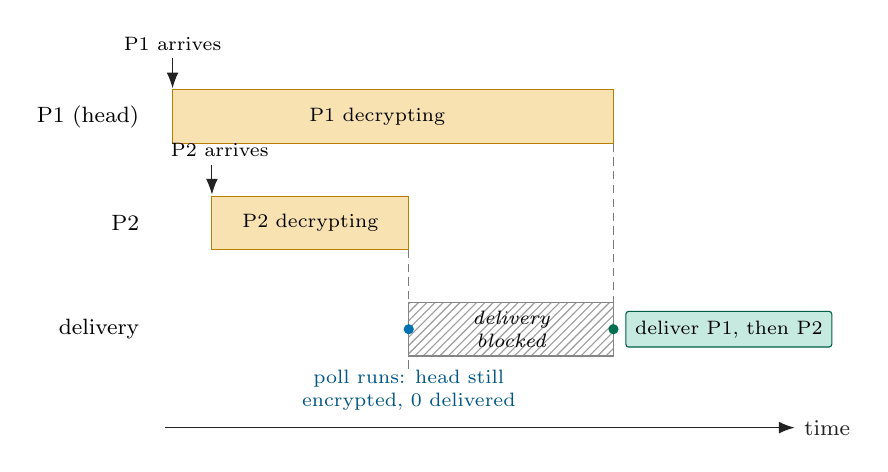
\begin{tikzpicture}[
  font=\sffamily\small,
  >={Latex[length=2mm]},
  enc/.style={draw=cAmber!80!black,fill=cAmber!30},
  don/.style={draw=cTeal!60!black,fill=cTeal!22},
  guide/.style={densely dashed,cInk!60},
  lane/.style={font=\footnotesize}
]
\def\ytop{2.7}   % P1 lane
\def\ymid{1.35}  % P2 lane
\def\ybot{0.0}   % delivery lane
\def\h{0.34}     % half-height of bars
\def\tCtwo{4.0}  % P2 completes
\def\tCone{6.6}  % P1 completes

% lane labels
\node[lane,anchor=east] at (0.7,\ytop) {P1 (head)};
\node[lane,anchor=east] at (0.7,\ymid) {P2};
\node[lane,anchor=east] at (0.7,\ybot) {delivery};

% P1 decrypt bar (long): amber then teal cap at completion
\fill[enc] (1.0,\ytop-\h) rectangle (\tCone,\ytop+\h);
\fill[don] (\tCone-0.35,\ytop-\h) rectangle (\tCone,\ytop+\h);
\draw[enc] (1.0,\ytop-\h) rectangle (\tCone,\ytop+\h);
\node[font=\scriptsize] at (3.6,\ytop) {P1 decrypting};

% P2 decrypt bar (short): completes earlier
\fill[enc] (1.5,\ymid-\h) rectangle (\tCtwo,\ymid+\h);
\fill[don] (\tCtwo-0.35,\ymid-\h) rectangle (\tCtwo,\ymid+\h);
\draw[enc] (1.5,\ymid-\h) rectangle (\tCtwo,\ymid+\h);
\node[font=\scriptsize] at (2.75,\ymid) {P2 decrypting};

% arrival ticks
\draw[->,cInk] (1.0,\ytop+\h+0.4) -- (1.0,\ytop+\h+0.02);
\node[font=\scriptsize,anchor=south] at (1.0,\ytop+\h+0.38) {P1 arrives};
\draw[->,cInk] (1.5,\ymid+\h+0.4) -- (1.5,\ymid+\h+0.02);
\node[font=\scriptsize,anchor=south] at (1.6,\ymid+\h+0.38) {P2 arrives};

% completion guides
\draw[guide] (\tCtwo,\ymid-\h) -- (\tCtwo,\ybot-0.5);
\draw[guide] (\tCone,\ytop-\h) -- (\tCone,\ybot-\h);

% delivery lane: blocked interval (hatched) between P2 and P1 completion
\fill[pattern=north east lines,pattern color=cInk!45]
     (\tCtwo,\ybot-\h) rectangle (\tCone,\ybot+\h);
\draw[cInk!55] (\tCtwo,\ybot-\h) rectangle (\tCone,\ybot+\h);
\node[font=\scriptsize\itshape,align=center] at (5.3,\ybot) {delivery\\blocked};

% event: poll runs at P2 completion, delivers nothing (label below the lane)
\node[circle,fill=cBlue,inner sep=1.3pt] at (\tCtwo,\ybot) {};
\node[font=\scriptsize,anchor=north,align=center,text=cBlue!75!black]
     at (\tCtwo,\ybot-\h-0.06) {poll runs: head still\\encrypted, 0 delivered};

% event: at P1 completion, both delivered in order
\node[circle,fill=cTeal!70!black,inner sep=1.3pt] at (\tCone,\ybot) {};
\node[don,rounded corners=1pt,anchor=west,font=\scriptsize] at (\tCone+0.15,\ybot)
     {deliver P1, then P2};

% time axis
\draw[->,cInk] (0.9,\ybot-1.25) -- (8.9,\ybot-1.25)
     node[anchor=west,font=\footnotesize]{time};

\end{tikzpicture}
\end{document}
